\section{Time Frequency Analysis}
Short Time Fourier Trasnform is a technique which is widely used and very useful for analysis of signals with a time varying spectral characteristics. STFT is used for analysis of respiratory signals since they have a nonstationary nature. 
\begin{equation}
X_m(f) = \sum_{n=-\infty}^{\infty}x(n)w(n-mR)e^{-j2\pi fn}
\label{STFT}
\end{equation} \par
STFT is defined in \eqref{STFT}. It can be seen as a sliding Fourier Transform (FT) \cite{stft-first}. In this equation, $R$ is hop size and $w$ is the window function which zero outside of a predefined range and is used to pick the part of signal which will be input of FT and smooth the signal to make it stationary. The window is an important parameter for STFT, it is the effective parameter to adjust time-frequency resolution. First of all, the window length must be so small that it must ensure that the selected portion is stationary. There is also a trade-off between resolution in time and resolution in frequency, this trade-off is also controlled with window length. As the  window length increases the frequency resolution increases and the time resolution decreases. So, for wideband signals one can use smaller window lengths whereas for narrowband signals greater window lengths may be used. \par
The output of STFT operation is a two dimensional complex matrix, which describes the magnitude and phase of frequency band component. For most of the time and for respiratory sounds too, we need the magnitude information and we convert the complex matrix to a real matrix which will give information about energy directly. The resulting matrix is usually visualized by a heatmap as in \ref{fig:sound_flow_specgram}.
\begin{figure}
	\begin{center}
		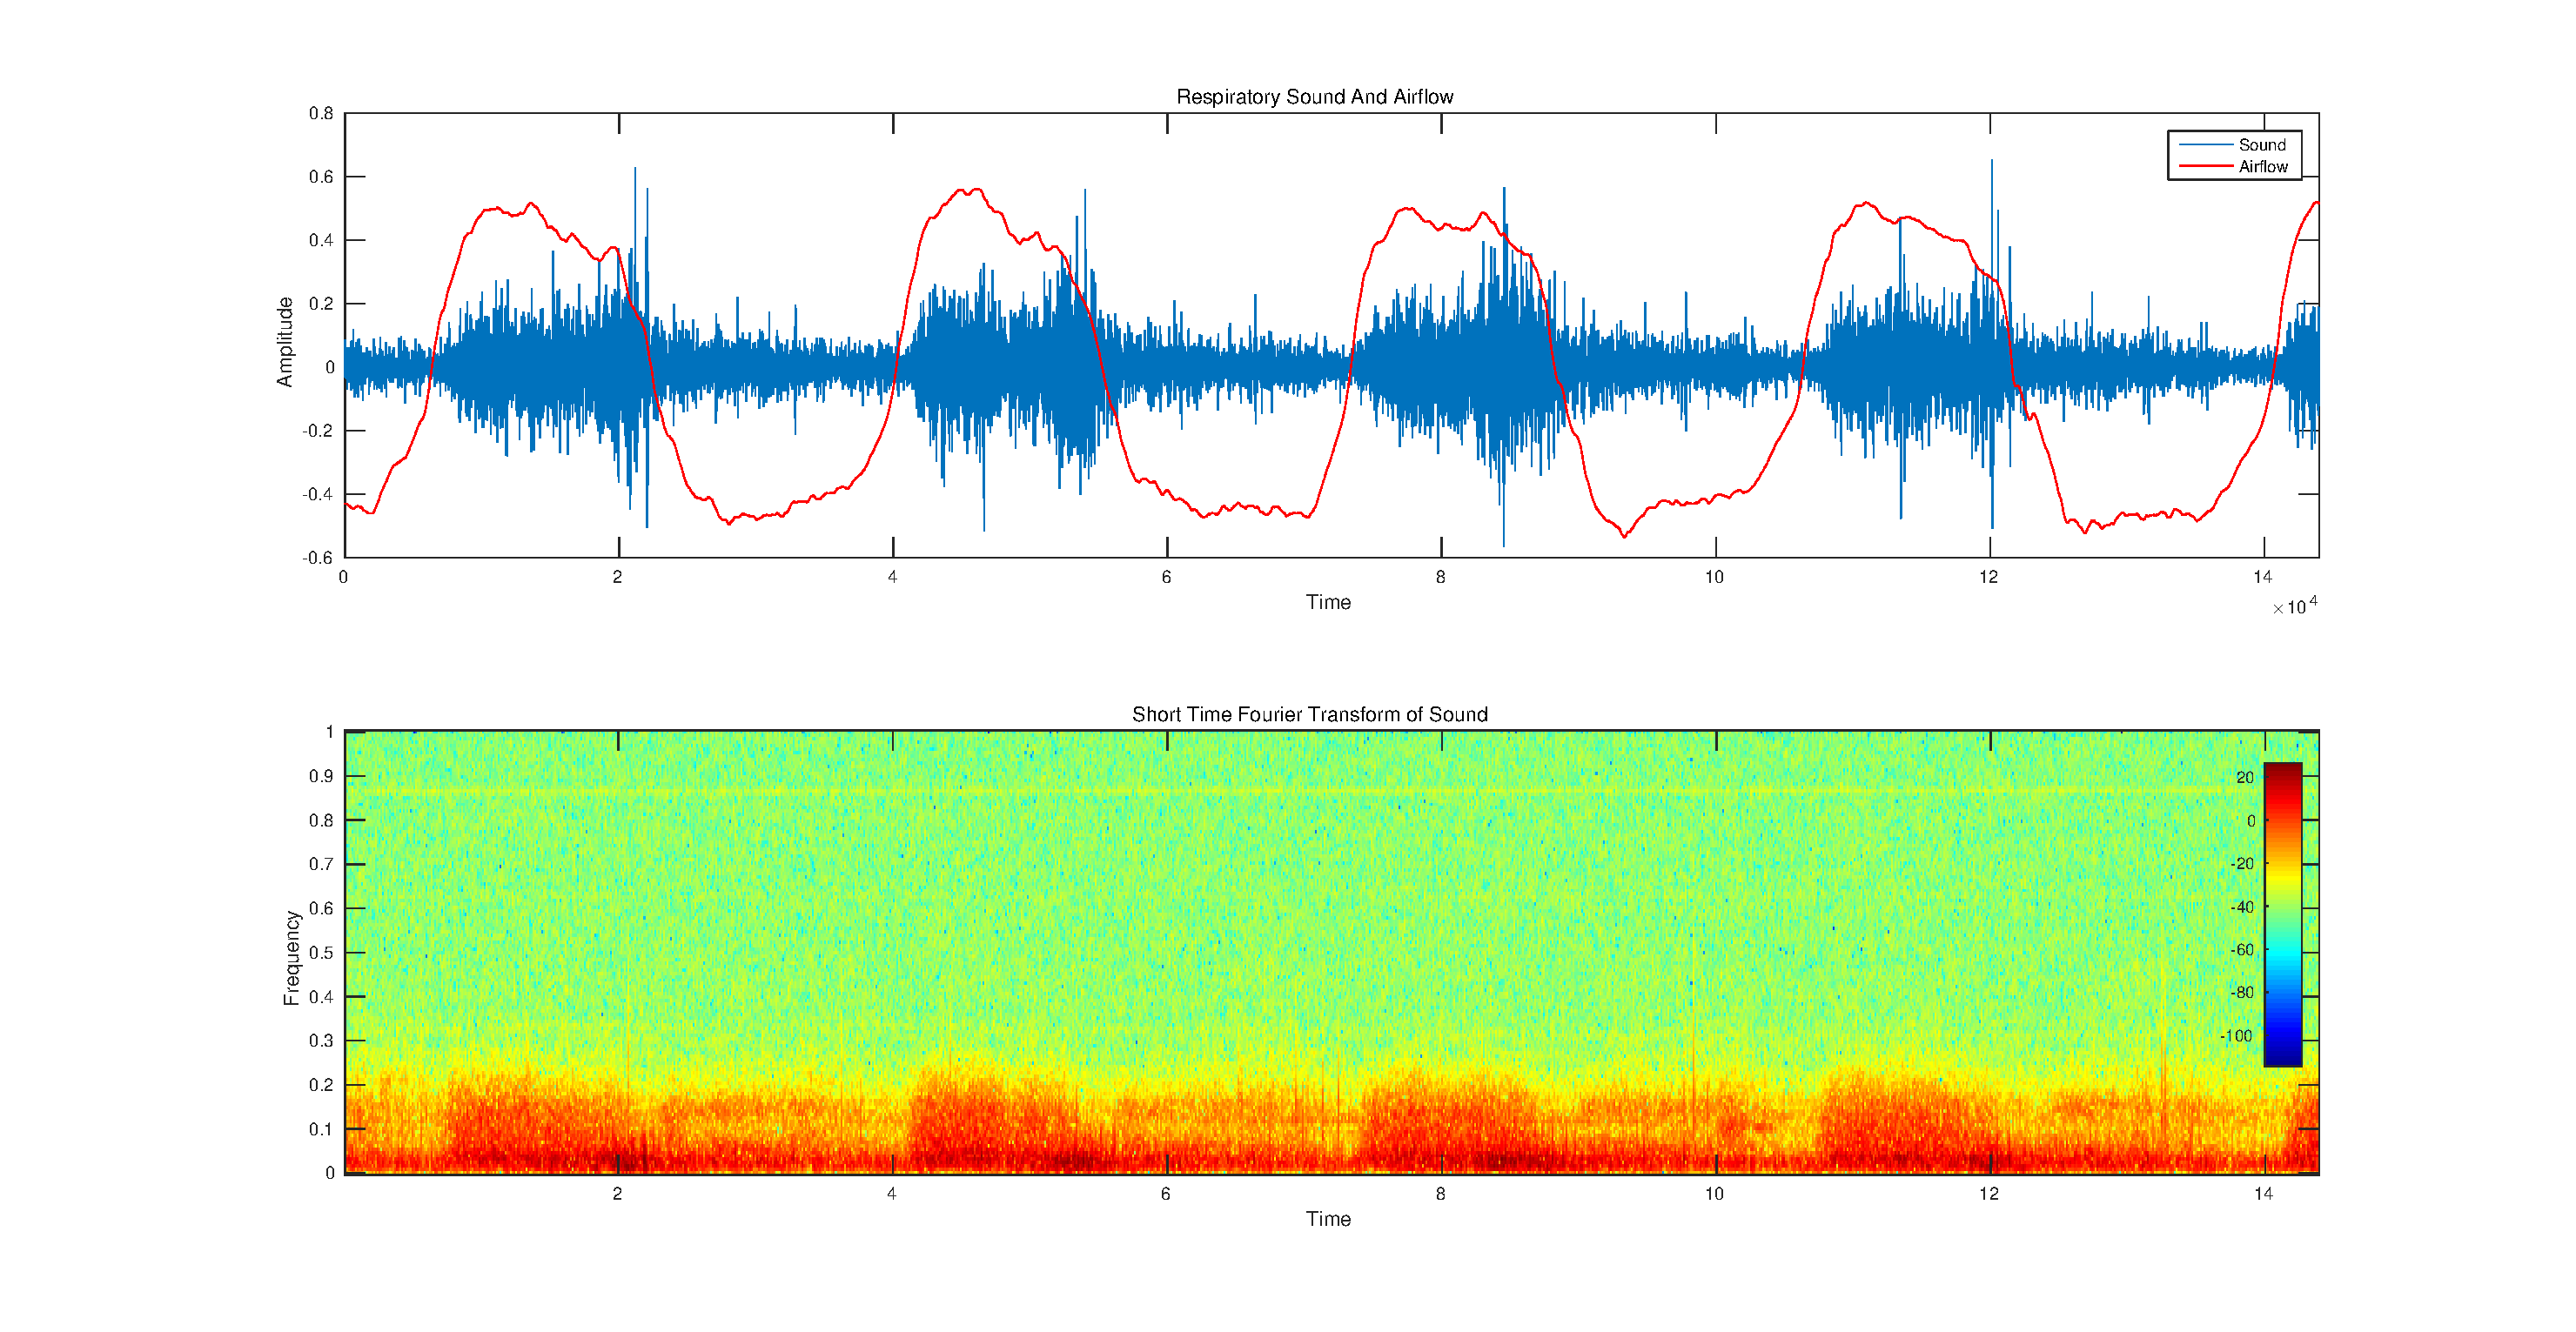
\includegraphics[width=\textwidth]{figures/sound_flow_specgram.eps}
		\caption{A respiratory sound, corresponding airflow and STFT magnitude plot}
		\label{fig:sound_flow_specgram}
	\end{center}
\end{figure} \par
When we look at figure \ref{fig:sound_flow_specgram}, respiratory sound, magnitude plot of its STFT and corresponding airflow we can see a trend seems related to airflow in evolution of some horizontal lines. They correspond to the energy at a frequency band over the time. We will run experiments to test the correlation between the evolution of energy at each frequency band with the airflow. We will tune STFT by tweaking the window type, window length and number of FFT bins in Experiment \& Results. 

